\documentclass[a4paper,11pt]{article}
\usepackage[utf8]{inputenc}
\usepackage{amssymb}
\usepackage{amsmath} 
\usepackage{enumerate}
\usepackage{graphicx}
\usepackage[font=small,labelfont=bf]{caption}
\graphicspath{ {./img/} }
\newcommand{\appropto}{\mathrel{\vcenter{
  \offinterlineskip\halign{\hfil$##$\cr
    \propto\cr\noalign{\kern2pt}\sim\cr\noalign{\kern-2pt}}}}}
\DeclareMathOperator*{\argmax}{arg\!\max}
\DeclareMathOperator*{\argmin}{arg\!\min}
\DeclareMathOperator*{\var}{var}
\DeclareMathOperator*{\nbr}{nbr}
\newcounter{exercise}
\setcounter{exercise}{0}
\newcounter{subexercise}
\newcommand*{\exercise}[1][]{
  \subsection*{Exercise
    \ifx/#1/\stepcounter{exercise}\arabic{exercise}
    \else#1\fi
  }
  \setcounter{subexercise}{0}
}
\newcommand*{\subexercise}[1][]{
  \par{
    \noindent{\ifx/#1/\protect\stepcounter{subexercise}\alph{subexercise}\else#1\fi.\quad}
  }
}
\title{Chapter 21}
\author{stevenjin8}
\date{June 28, 2021}

\begin{document}

	\maketitle

	\section*{Exercises}
	\exercise
	\begin{figure}[t]
	\centering
	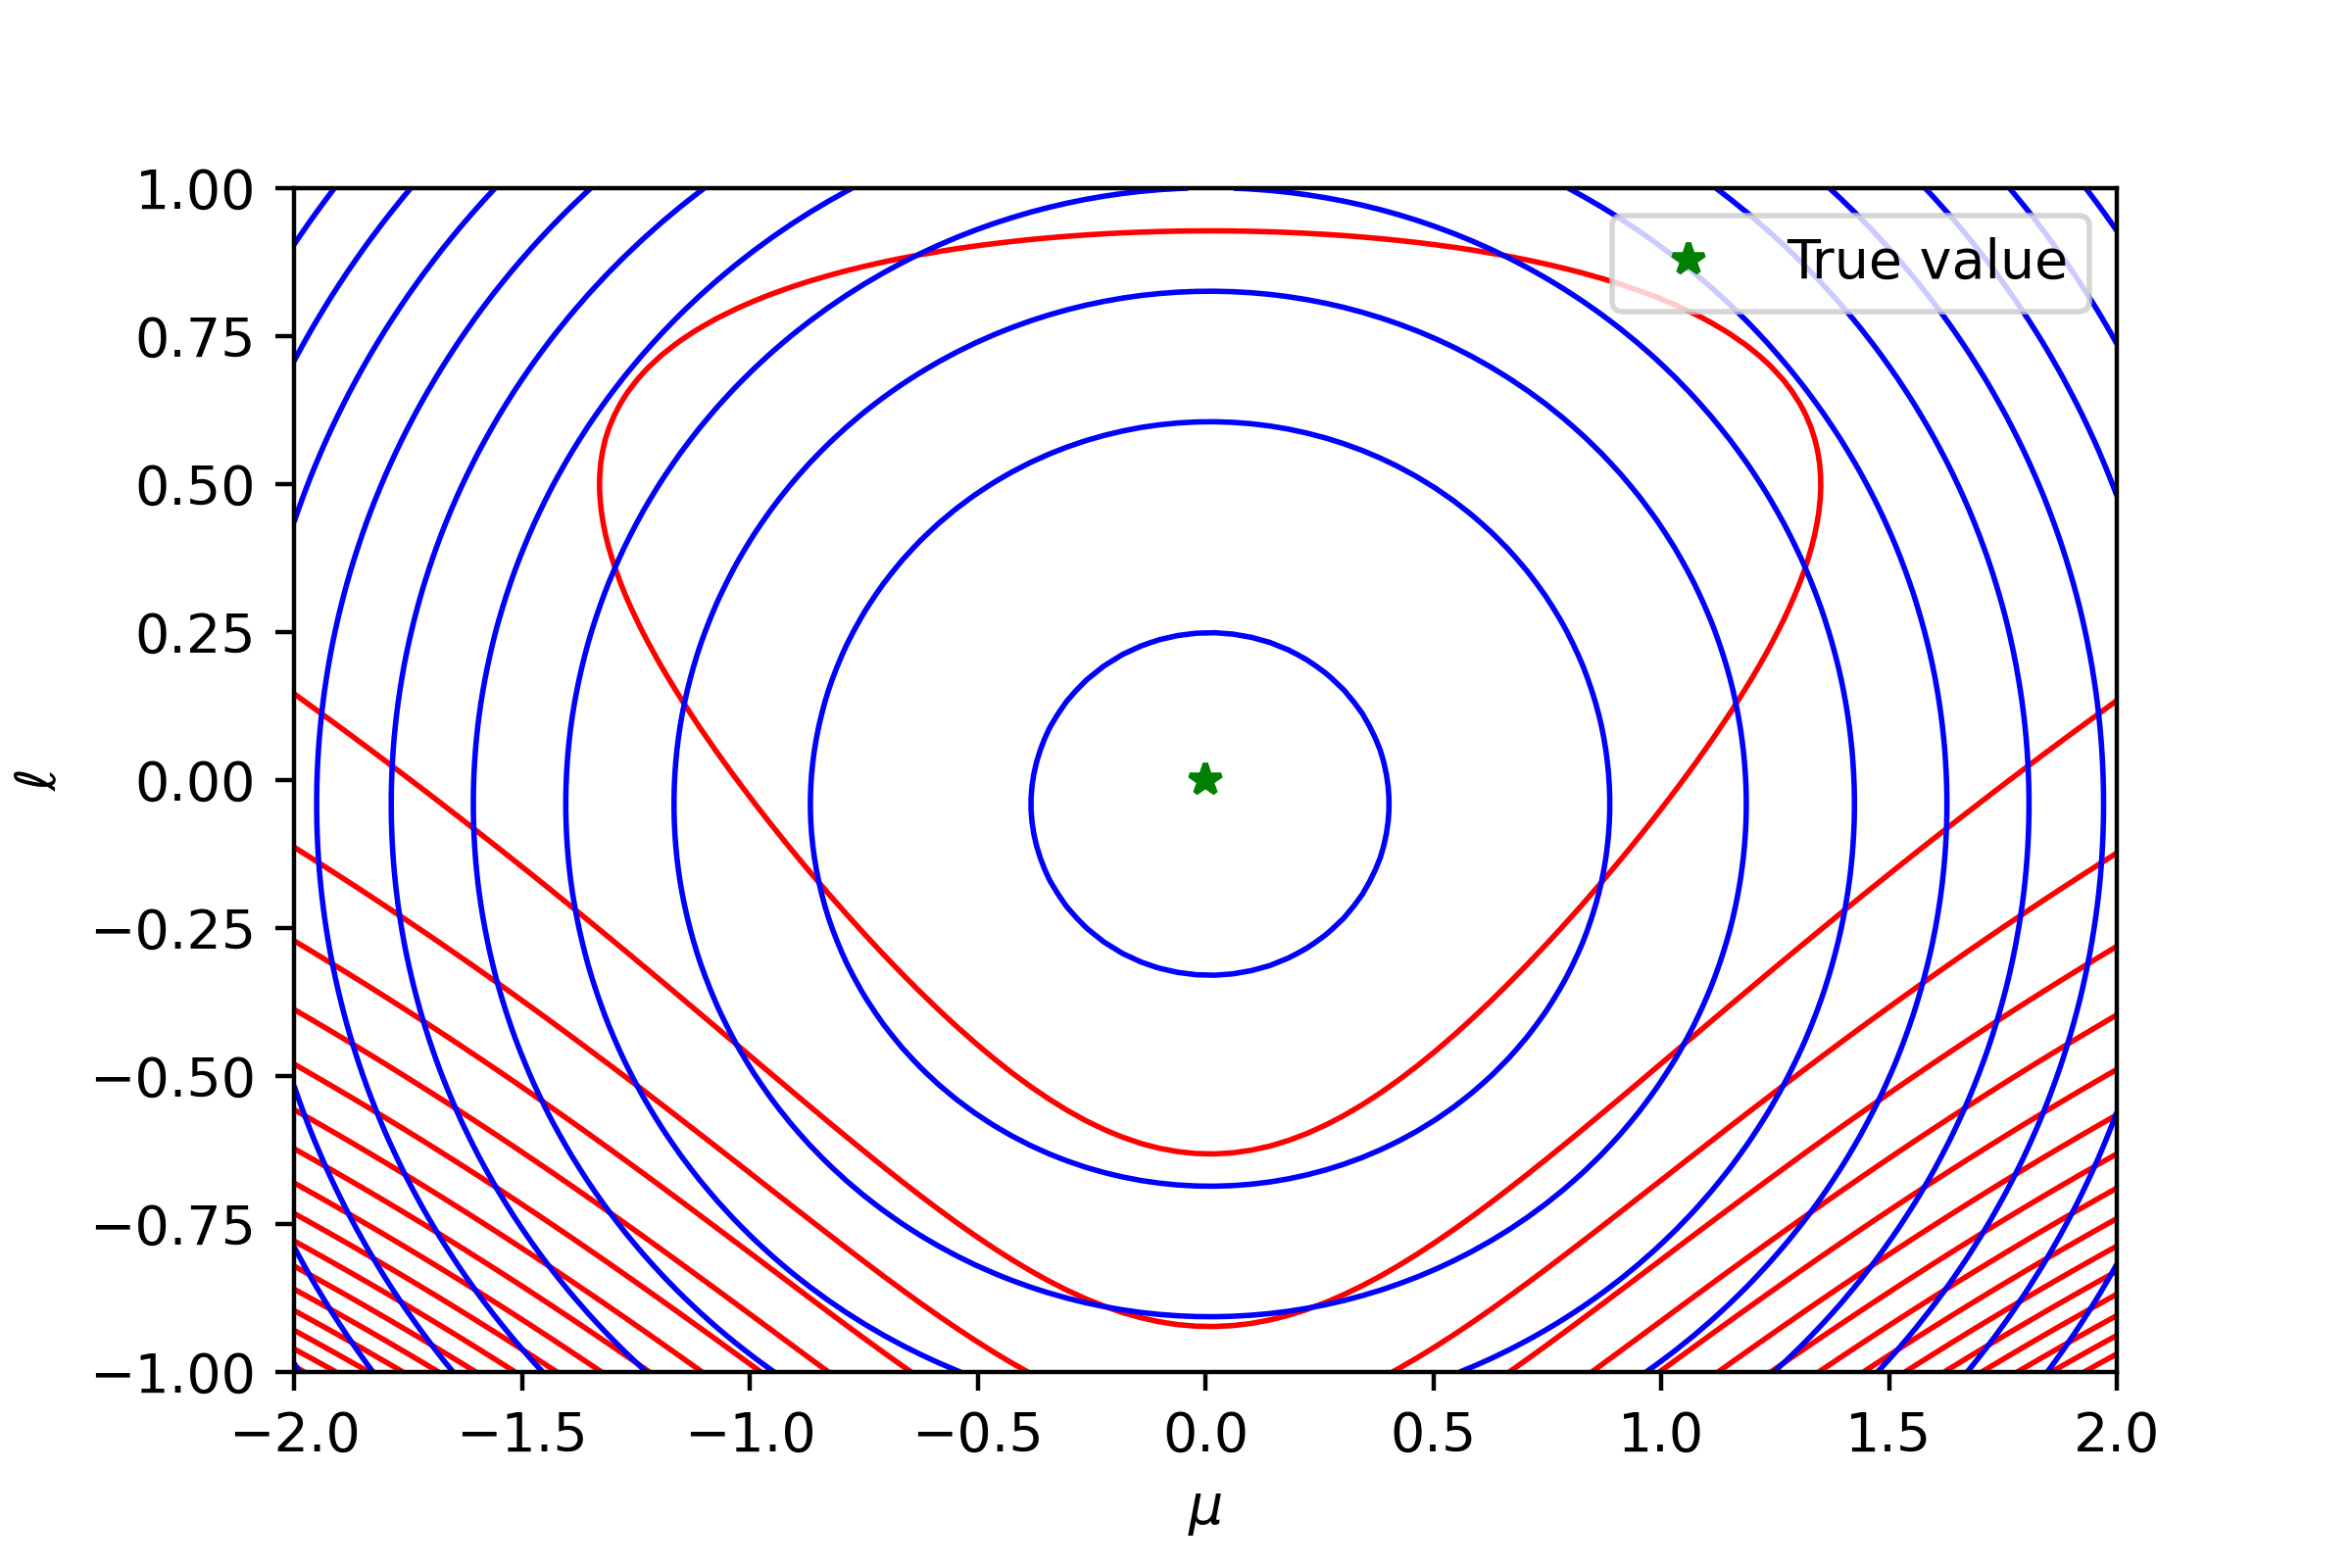
\includegraphics[width=10cm]{gaussian-posterior-approx.png}
	\caption{True log posterior (red) vs Laplacian approximation (blue). Data are 15 samples from a
	unit normal distribution ($\mu, \ell=0$).}
	\end{figure}

	This exercise confused me very much because I thought it was asking to use Laplace distribution
	to approximate the posterior, rather than a Laplacian approximation of the posterior.

	Following the presentation in section 8.4.1, the posterior is given by
	\begin{equation}
		p( \mu, \ell | \mathcal{D} ) = \frac1Z e ^ { -E( \mu, \ell )},
	\end{equation}
	where
	\[
		E( \mu, \ell ) = n \log\sigma + \frac{n}{ 2\sigma^2 }
		\left( s^2 + ( \overline{x} - \mu )^2 \right ),
	\]
	which is just equation 21.203 negated.

	Finding the gradient is straightforward:
	\begin{align*}
		\frac{ \partial E }{ \partial\mu } &= -\frac{ n( \overline{x} - \mu )}{ \sigma^2 } \\
		\frac{ \partial E }{ \partial\ell }
		&= \frac\partial{ \partial\ell } \left[
			n \ell + e ^ { -2\ell } \frac{n}2
			\left( s^2 + ( \overline{x} - \mu )^2 \right)
		\right] \\
		&= n - e ^ { -2\ell } n \left( s^2 + ( \overline{x} - \mu )^2 \right) \\
		&= n - \frac{
			n \left( s^2 + ( \overline{x} - \mu )^2 \right)
		}{ \sigma^2 }.
	\end{align*}

	The Hessian is also pretty easy to compute:
	\begin{align*}
		\frac{ \partial^2E }{ \partial\mu^2 } &= \frac{ n\overline{x} }{ \sigma^2 } \\
		\frac{ \partial^2E }{ \partial\mu \partial\ell }
		&= \frac{ 2n( \overline{x} - \mu )}{ \sigma^2 } \\
		\frac{ \partial^2E }{ \partial\ell^2 } &=
		\frac\partial{ \partial\ell } n - e ^ { -2\ell } n \left(
			s^2 + ( \overline{x} - \mu )^2
		\right) \\
		&= 2\frac{ n \left( s^2 + ( \overline{x} - \mu )^2 \right)}{ \sigma^2 }. \\
	\end{align*}

	Setting the first derivatives (i.e. the gradient) to $\mathbf0$ and solving gives
	\[
		\mu^* = \overline{x}, \ell^* = \log s.
	\]
	Thus, the Hessian  of $E$ at  $\mu=\mu^*, \ell=\ell^*$ is
	\[
	\mathbf{H} = \begin{bmatrix}
	  \frac{n}{s^2} & 0 \\
	  0 & 2n \\
	\end{bmatrix}
	\]

	We can approximate $E$ with
	\[
	E( \boldsymbol{\theta} ) \approx E( \boldsymbol{\theta}^* )
	+ \frac12 ( \boldsymbol{\theta} - \boldsymbol{\theta}^* )^T \mathbf{H}
	( \boldsymbol{\theta} - \boldsymbol{\theta}^* )
	\]
	where $\boldsymbol{\theta} = (\mu, \ell)$. Finally, we plug this into equation 1:
	\begin{align*}
		p( \boldsymbol{\theta} | \mathcal{D} ) &\appropto e ^ {
			-E( \boldsymbol{\theta}^* )
			- \frac12 ( \boldsymbol{\theta} - \boldsymbol{\theta}^* )^T \mathbf{H}
			( \boldsymbol{\theta} - \boldsymbol{\theta}^* )
		 } \\
	&\propto e ^ {
	  -\frac12  ( \boldsymbol{\theta} - \boldsymbol{\theta}^*)^T \mathbf{H}
	   ( \boldsymbol{\theta} - \boldsymbol{\theta}^*)
	}
	\end{align*}
	We can see that
	\[
		p(\mu, \ell) \approx
		\mathcal{N}\left( \boldsymbol{\theta} | \boldsymbol{\theta}^*, \mathbf{H}^{-1} \right).
	\]
	See Figure 1 for a visualization.

	I found the way the author suggested to this problem to be a bit unintuitive because it makes
	you think that the Hessian in equation 21.206 is the inverse of the covariance matrix. However,
	this cannot be true since the entries on the diagonal would be negative.

	\setcounter{exercise}{5}
	\exercise
	The goal here is to minimize
	\[
		\mathbb{KL} ( q_i \parallel \tilde{p}_i ) = \sum\limits_{ x \in \{ -1, 1 \} }
		q_i(x) \log\frac{ q_i(x) }{ \tilde{p}_i( x ) }.
	\]
	This can be achieved by setting $q_i(x) \propto \tilde{p}_i(x)$. Thus, we have
	\[
		q_i( x=1 ) = \frac{ e ^ { m_i + L^+ }}{ e ^ { m_i + L^+ } + e ^ { -m_i + L^- }}.
	\]
	where $m_i, L^+,$ and $L^-$ have the same meanings as in section 21.3.2. The result follows from
	equations 21.46-21.50.

	\exercise
	\begin{align*}
		\mathbb{KL}( p \parallel q ) &= \sum\limits_{x,y} p( x, y )
		\log \frac{ p( x,y )}{ q( x )q( y ) } \\
		&= \sum\limits_{x,y} p( x, y ) ( \log p( x, y ) - \log q( x ) - \log q( y )) \\
		& = \sum\limits_{x,y} p( x, y )\log p( x, y )
		- \sum\limits_y p( y ) \log q( y ) - \sum\limits_x p( x ) \log q( x ).
	\end{align*}
	We minimize this by setting $q( x ) = p( x )$ and $q( y ) = p( y )$.

	Following section 21.2.2,  $p( x, y ) = 0  \implies q( x )q( y ) = 0$. It follows that the three local
	minima are
	\begin{align*}
		&q( x ) = q( y ) = [ 0.5, 0.5, 0, 0 ] \\
		&q( x ) = q( y ) = [ 0, 0, 1, 0 ] \\
		&q( x ) = q( y ) = [ 0, 0, 0, 1 ].
	\end{align*}
	Which have a KL divergence of $\log2, \log4$, and  $\log4$ respectively.

	By setting $q( x, y ) = p( x )p( y )$, the KL divergence diverges.
\end{document}
